\documentclass[10pt]{report}
\usepackage{epsf}
\usepackage{amsmath}
\usepackage{amssymb}
\usepackage{float}
\usepackage{palatino}
\usepackage[pdftex]{graphics}
\usepackage{fancyhdr}
\usepackage[pdftex]{graphicx}
\usepackage{hyperref}
\parindent 0in
\parskip 1ex
\oddsidemargin  0in
\evensidemargin 0in
\textheight 8.5in
\textwidth 6.5in
\topmargin -0.25in

\pagestyle{fancy}
\fancyhf{}
\fancyhead[L]{\bf BME354L - Palmeri - Spring 2013}
\fancyhead[R]{{\bf Arduino Project}}
%\fancyfoot[L]{LICENSE: CC BC-NC-SA 3.0 ({\tt http://creativecommons.org/licenses/by-nc-sa/3.0/})}
\fancyfoot[C]{\thepage}

\title{Tips for Using Thermocouples}
\author{Will Scheideler}
\begin{document}

\section*{Tips for Using Thermocouples}

\subsection*{Introduction}
Hi and welcome to BME 354! This class integrates many concepts from Electrical Engineering and Biomedical Engineering, from circuit design to signal processing. This semester, we are putting a greater emphasis on microcontrollers and embedded programming, in light of how ubiquitous they are. Today, almost every electronic device, from toaster ovens to heart rate monitors, uses some sort of microcontroller. For the first time, BME 354 will introduce a final project involving the Arduino Uno hardware platform. Throughout the semester, we will post a series of small tutorials to get you comfortable working with the Arduino Uno so the project will be a very natural transition.
\par
I realize those of you taking this class come from different backgrounds-some may be ECE’s with a strong background in programming, others may be BME’s with little interest in this area. For the ECE’s, some of the content in these tutorial may be very easy for you, but I still encourage you to play around with the Arduino and maybe you’ll discover something cool. For the BME’s, I hope this series of tutorials generates some interest in embedded systems, at the very least bestow some general knowledge about microcontrollers that is very important in the biomedical engineering industry today.

\subsection*{What is a microcontroller?}

A microcontroller is essentially a small computer. It is a small integrated circuit (as opposed to a circuit with discrete components, an IC has all its circuit components printed onto a single chip) that is able to run computer code, take inputs, and control outputs. As a result of being printed, IC’s are often really very small (you’ve already worked with IC’s in the form of the AD620 and LF353 op-amps). In contrast to the microprocessors used in say your laptop, microcontrollers are designed for embedded applications (this means they usually perform a very specific task, are lower power and lower cost). 
\par
They are often used in devices that don’t necessarily need all the functionality of your laptop’s Intel Core i7; for example, a remote control only needs to be able to detect the user’s button presses, transmit some sort of signal to your television, and do all this with as long a battery life as possible. Some devices, such as a toaster oven, were originally built without microcontrollers at all. However, as you will see, microcontrollers have many benefits: they are cheap, are often more reliable than mechanical components, and can be programmed for greater functionality. Many medical devices can be categorized as embedded systems, with a specific function to perform. With the advent of many portable and implanted medical devices, specialized system-on-a-chip designs are becoming increasingly relevant. The Arduino Uno platform uses an ATMega328P microcontroller. The Uno is pictured in Figure 1 and that long, black component is the microcontroller.

\begin{figure}[H]
\centering
   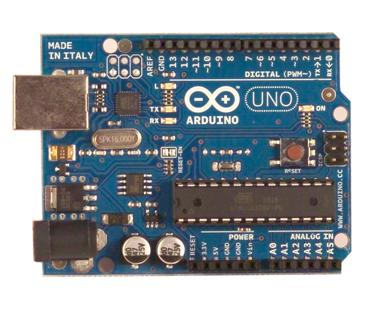
\includegraphics[width=0.7\textwidth]{arduino.jpg}
    \caption{A view of the Arduino board.}
\end{figure}

\subsection*{Microcontroller Breakdown}

So, how does a microcontroller work? How do we characterize its performance and capabilities? Here are some terms that you should be familiar with when working with the Arduino. 

 \begin{itemize}
\item \textbf{Operating Voltage} - This is supply voltage (Vdd) of the development board; the USB cable or power jack will supply this voltage to the board. The Arduino Uno’s operating voltage is 5V; another common operating voltage is 3.3V (useful for devices powered by 3.7V LiI cells, i.e. your cellphone). The Arduino is also built with a Vin pin that allows for an alternative supply voltage.
  
\item \textbf{Frequency} – Also called the clock. This is a signal that oscillates between +/- Vdd that controls how many instructions the microcontroller will execute every second. On the Arduino Uno, the clock is 16 MHz and is dictated by a ceramic resonator (a piezoelectric component that oscillates when you pass a voltage through it). For comparison, your laptop is probably clocked at around 2 GHz.

\item Memory
\begin{itemize}

\item Flash – This is kind of like the hard drive on your computer. It’s non-volatile memory, meaning that when you turn the power off, the data stored in this memory will not be erased. This is where the program and your variables are stored.

\item EEPROM – This is also nonvolatile memory. It is used to store long term information. It can only be accessed using read() and write().

\item SRAM – This is like the ram in your computer, so it is volatile memory, meaning that it will be cleared if your turn the power off. It is used by the Arduino to perform calculations and operations on your variables.

\end{itemize}
\end{itemize}

\subsection*{Arduino I/O}

I/O stands for input/output. Input and output refer to the signals that are transmitted to and from an embedded systems. Inputs to the microcontroller may originate as signals of nearly any kind (i.e. pressure, temperature, height, force, magnetic field, conductivity, etc). The good news is that transducers exist to convert these signals to voltages. A microcontroller then reads the voltage at an input pin and processes these voltage signals before giving feedback to the system. Feedback originates as voltage at an output pin of the microcontroller. Transducers convert this signal back into other forms of energy. Figure 2, below, illustrates this process.

%\begin{figure}[H]
%\centering
%   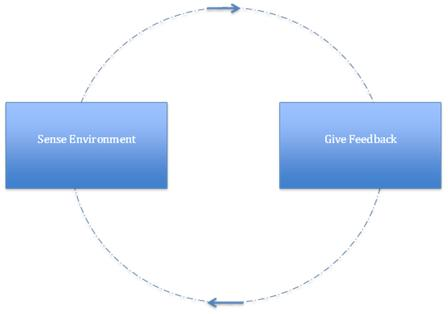
\includegraphics[width=0.8\textwidth]{feedback.jpg}
%    \caption{Figure 2: Schematic of the general scheme of an embedded system.}
%\end{figure}

\begin{itemize}
\item 
\end{itemize}




\end{document}